\subsubsection{UC26 - Selezione DBMS}\label{UC26}

\begin{figure}[H]
  \centering
  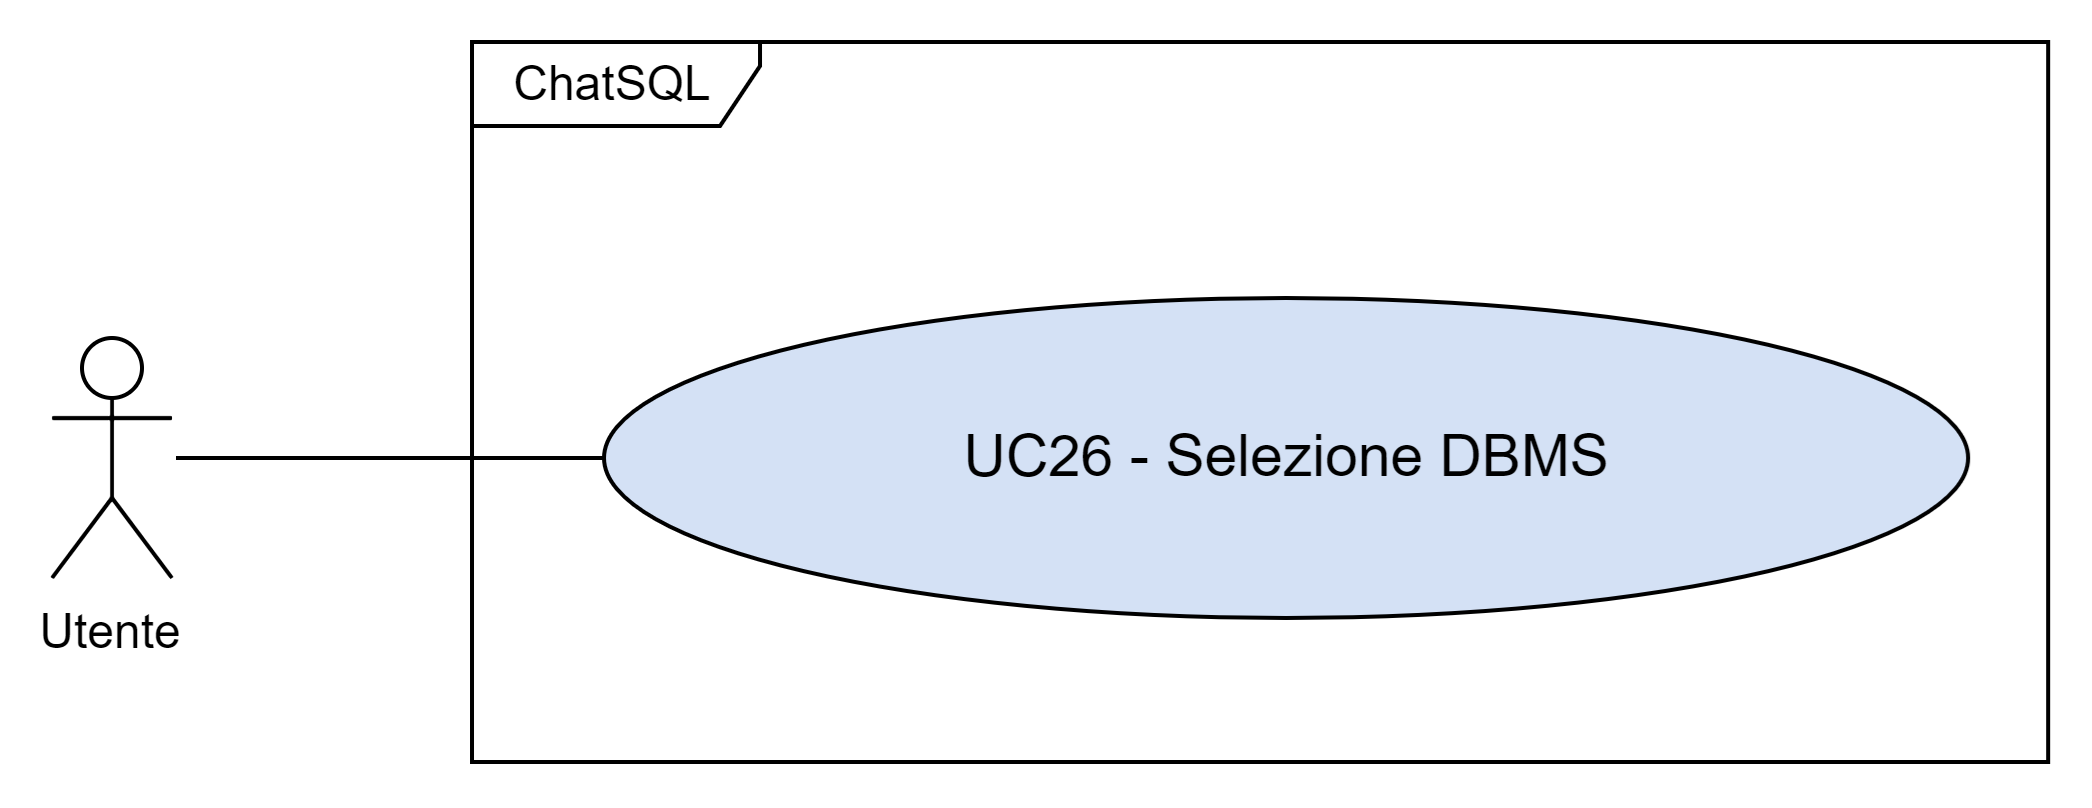
\includegraphics[width=0.90\textwidth]{assets/uc26.png}
  \caption{UC26}
\end{figure}

\paragraph*{Descrizione}
L'Utente seleziona un \glossario{DBMS} tra quelli disponibili. La scelta del DBMS è un passaggio chiave nella generazione del \glossario{prompt}. Sebbene \glossario{SQL} sia un linguaggio standard, esistono variazioni specifiche per ogni DBMS. Per garantire che un \glossario{LLM} generi una \glossario{query} SQL corretta, il prompt deve indicare anche il DBMS di destinazione.

\paragraph*{Attori principali}
Utente

\paragraph*{Precondizioni}
\begin{itemize}
  \item L'applicazione è stata avviata con successo;
  \item L'Utente sta visualizzando correttamente la chat.
\end{itemize}

\paragraph*{Postcondizioni}
\begin{itemize}
  \item Il \glossario{DBMS} è stato selezionato correttamente.
\end{itemize}

\paragraph*{Trigger}
L'Utente vuole selezionare un \glossario{DBMS} per la generazione del \glossario{prompt}.

\paragraph*{Scenario principale}
\begin{enumerate}
  \item L'Utente sceglie un \glossario{DBMS} da una lista predefinita. La scelta è tra i seguenti DBMS:
    \begin{itemize}
      \item MySQL;
      \item MariaDB;
      \item PostgreSQL;
      \item Microsoft SQL Server;
      \item Oracle Database;
      \item SQLite.
    \end{itemize} 
\end{enumerate}